
%% \begin{figure*}
%%   \vspace{-0.3in}
%%   \centering
%%   \subfloat[\(N=2^2\)]{
%%     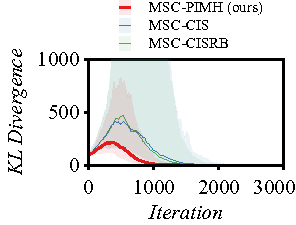
\includegraphics[scale=0.75]{figures/gaussian_01.pdf}
%%   }
%%   \subfloat[\(N=2^4\)]{
%%     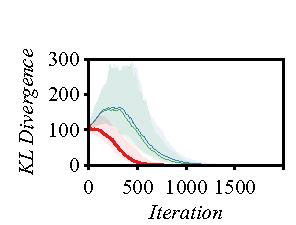
\includegraphics[scale=0.75]{figures/gaussian_02.pdf}
%%   }
%%   \subfloat[\(N=2^6\)]{
%%     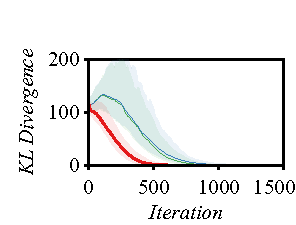
\includegraphics[scale=0.75]{figures/gaussian_03.pdf}
%%   }
%%   \caption{100-D isotropic Gaussian example with a varying computational budget \(N\).
%%     MSC-PIMH converges faster than MSC-CIS and MSC-CISRB regardless of \(N\).
%%     Also, the convergence of MSC-PIMH becomes more stable/monotonic as \(N\) increases.
%%     The solid lines and colored regions are the medians and 80\% percentiles computed from 100 repetitions.
%%   }\label{fig:gaussian}
%%   \vspace{-0.15in}
%% \end{figure*}

\vspace{-0.05in}
\section{Evaluations}\label{section:eval}

\begin{figure}[t]
\centering
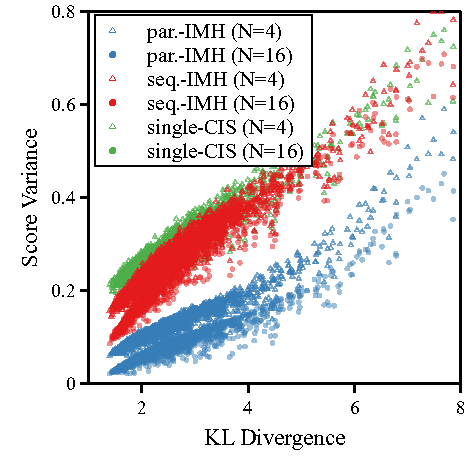
\includegraphics[scale=0.8]{figures/simulation_02.pdf}
\caption{Variance of score function estimated using the three estimators depending on \(N\) and the KL divergence.
Each point represent a random \(\vlambda\) where the score is evaluated.}\label{fig:simulation}
\end{figure}
%
\subsection{Numerical Simulation}
\paragraph{Experimental Setup}
We first present numerical simulation results of the three estimators.
We chose the target distribution \(p\left(\vz\right)\) to be a 10 dimensional white Gaussian.
We then randomly generated 2048 random \(q_{\vmu, \mSigma}(\vz)\) where \(\vmu\) is drawn from a multivariate Student's T distribution, and \(\mSigma = 1.5^2 \mI\).
Using the 2048 random \(q_{\vmu, \mSigma}\)s, we simulate 128 Markov-chains of length \(T=50\) and compute the bias and variance of the score function.

\paragraph{Results}
The variance results are shown in~\cref{fig:simulation}.
We do not present the bias as the three schemes were visually indistinguishable for all settings.
From the results, when the KL divergence is large, we can see that seq.-IMH and single-CIS do not benefit from increasing \(N\).
On the other hand, the parallel state estimator always benefit from increasing \(N\).

\subsection{Baselines and Implementation}
\paragraph{Implementation}
We implemented MSC with PIMH on top of the Turing~\citep{ge2018t} probabilistic programming framework.
Our implementation works with any model described in Turing, which automatically handles distributions with constrained support~\citep{JMLR:v18:16-107}.
We use the ADAM optimizer by~\citet{kingma_adam_2015} with a learning rate of 0.01 in all of the experiments.
We set the computational budget \(N=10\) and \(T=10^4\) for all experiments unless specified.

\vspace{-0.1in}
\paragraph{Considered Baselines}
We compare the following baselines.
\vspace{-0.1in}
\begin{enumerate}[noitemsep]
  \item[\ding{182}] \textbf{par.-IMH}: Score climbing with the parallel state estimator and the IMH kernel. 
  \item[\ding{183}] \textbf{seq.-IMH}: Score climbing with the sequential state estimator and the IMH kernel 
  \item[\ding{184}] \textbf{single-CIS}: Score climbing with the single state estimator and the CIS kernel~\citep{NEURIPS2020_b2070693}.
  \item[\ding{185}] \textbf{single-CISRB}: Rao-Blackwellized version of single-CIS~\citep{NEURIPS2020_b2070693}.
  \item[\ding{184}] \textbf{single-HMC}: Score climbing with the single state estimator and the HMC kernel.
  \item[\ding{186}] \textbf{SNIS}: adaptive IS using SNIS (as discussed in~\cref{section:ivi_previous}).
  \item[\ding{187}] \textbf{ELBO}: evidence lower-bound maximization with automatic differentiation VI~\citep{pmlr-v33-ranganath14, JMLR:v18:16-107} and the path derivative estimator~\citep{NIPS2017_e91068ff}.
\end{enumerate}
For ELBO, we use only a single sample as originally described by~\citet{NIPS2017_e91068ff}.
This also ensures a fair comparison against inclusive KL minimization methods since the iteration complexity of computing the ELBO gradient can be easily few orders of magnitude larger.
Finally, we only use single-HMC in the logistic regression experiment due to the high computational demands, 


\begin{table*}
  \centering
  \caption{Classification Accuracy and Log Predictive Density on Logistic Regression Problems}\label{table:logistic}
  \setlength{\tabcolsep}{3pt}
  \begin{threeparttable}
  \begin{tabular}{lcccccc}
    \toprule
     & \multicolumn{2}{c}{\textbf{\texttt{pima}}} & \multicolumn{2}{c}{\textbf{\texttt{heart}}} & \multicolumn{2}{c}{\textbf{\texttt{german}}} \\
    \cmidrule(lr){2-3}\cmidrule(lr){4-5}\cmidrule(lr){6-7}
    & Test Accuracy & Test LPD
    & Test Accuracy & Test LPD
    & Test Accuracy & Test LPD \\\midrule
    ELBO & \textbf{0.77 {\scriptsize(0.77, 0.77)}} & -0.53 {\scriptsize(-0.55, -0.51)} & 0.84 {\scriptsize(0.84, 0.84)} & \textbf{-0.40 {\scriptsize(-0.40, -0.39)}} & \textbf{0.77 {\scriptsize(0.77, 0.77)}} & -0.54 {\scriptsize(-0.58, -0.50)}  \\\arrayrulecolor{black!30}\midrule
    par.-IMH (ours) & \textbf{0.77 {\scriptsize(0.77, 0.77)}} & \textbf{-0.51 {\scriptsize(-0.51, -0.50)}} & \textbf{0.85 {\scriptsize(0.84, 0.85)}} & \textbf{-0.40 {\scriptsize(-0.40, -0.40)}} & \textbf{0.77 {\scriptsize(0.77, 0.77)}} & \textbf{-0.50 {\scriptsize(-0.50, -0.50)}} \\
    seq.-IMH & 0.67 {\scriptsize(0.65, 0.69)} & -0.71 {\scriptsize(-0.76, -0.65)} & 0.79 {\scriptsize(0.78, 0.80)} & -0.45 {\scriptsize(-0.46, -0.44)} & 0.76 {\scriptsize(0.76, 0.76)} & -0.51 {\scriptsize(-0.51, -0.51)} \\
    single-CIS & 0.69 {\scriptsize(0.67, 0.71)} & -0.68 {\scriptsize(-0.73, -0.62)} & 0.79 {\scriptsize(0.78, 0.80)} & -0.46 {\scriptsize(-0.48, -0.44)} & 0.76 {\scriptsize(0.75, 0.76)} & -0.51 {\scriptsize(-0.52, -0.51)} \\
    single-CISRB & 0.71 {\scriptsize(0.69, 0.72)} & -0.62 {\scriptsize(-0.67, -0.58)} & 0.80 {\scriptsize(0.79, 0.81)} & -0.44 {\scriptsize(-0.45, -0.43)} & 0.76 {\scriptsize(0.76, 0.76)} & -0.52 {\scriptsize(-0.52, -0.51)} \\
    single-HMC & 0.75 {\scriptsize(0.75, 0.75)} & -0.52 {\scriptsize(-0.53, -0.52)} & 0.80 {\scriptsize(0.79, 0.81)} & -0.45 {\scriptsize(-0.46, -0.44)} & \textbf{0.77 {\scriptsize(0.76, 0.77)}} & -0.61 {\scriptsize(-0.72, -0.49)} \\
    SNIS & 0.72 {\scriptsize(0.71, 0.72)} & -0.59 {\scriptsize(-0.61, -0.57)} & 0.78 {\scriptsize(0.77, 0.79)} & -0.46 {\scriptsize(-0.48, -0.45)} & 0.75 {\scriptsize(0.75, 0.76)} & -0.52 {\scriptsize(-0.52, -0.52)} \\\bottomrule
  \end{tabular}
  \begin{tablenotes}
    \item[*]{\footnotesize LPD denotes the average log predictive density.}
    \item[*]{\footnotesize The numbers in the parentheses denote the 80\% bootstrap confidence intervals.}
  \end{tablenotes}
  \end{threeparttable}
\end{table*}

%%% Local Variables:
%%% TeX-master: "master"
%%% End:

%% \subsection{Isotropic Gaussian}
%% We first perform experiments with an 100-D isotropic multivariate Gaussian distribution.
%% With Gaussian distributions, convergence can be evaluated exactly since their KL divergence is available in a closed form.
%% We compare the performance of MSC-PIMH, MSC-CIS, and MSC-CISRB with respect to the \(N\) (number of proposals for MSC-CIS, MSC-CISRB; number of parallel chains for MSC-PIMH).
%% The results are shown in~\cref{fig:gaussian}.
%% While MSC-PIMH shows some level of overshoot wih \(N=4\), it shows monotonic convergence with larger \(N\).
%% On the other hand, both MSC-CIS and MSC-CISRB overshoots even with \(N=64\).
%% This clearly shows that our PIMH kernel enjoys better gradient estimates compared to the CIS kernel.

\subsection{Hierarchical Logistic Regression}\label{section:logistic}
\vspace{-0.05in}
\paragraph{Experimental Setup}
We evaluate MSC-PIMH on logistic regression with the Pima Indians diabetes (\textbf{\texttt{pima}}, \(\vz \in \mathbb{R}^{11}\),~\citealt{smith_using_1988}), German credit (\textbf{\texttt{german}}, \(\vz \in \mathbb{R}^{27}\)), and heart disease (\textbf{\texttt{heart}}, \(\vz \in \mathbb{R}^{16}\),~\citealt{detrano_international_1989}) datasets obtained from the UCI repository~\citep{Dua:2019}.
10\% of the data points were randomly selected in each of the 100 repetitions as test data.

\vspace{-0.1in}
\paragraph{Probabilistic Model}
Instead of the usual single-level probit/logistic regression models used in VI, we choose a more complex hierarchical logistic regression model 
%
\begin{align*}
\sigma_{\beta}, \sigma_{\alpha} &\sim \mathcal{N}^{+}(0, 1.0) \\
\symbf{\beta} &\sim \mathcal{N}(\symbf{0},\, \sigma_{\beta}^2 \mI) \\
p &\sim \mathcal{N}(\vx_i^{\top}\symbf{\beta} + \alpha,\, \sigma_{\alpha}^2) \\
y_i &\sim \text{Bernoulli-Logit}\,(p)
\end{align*}
%
where \(\mathcal{N}^+(\mu, \sigma)\) is a positive constrained normal distribution with mean \(\mu\) and standard deviation \(\sigma\), \(\vx_i\) and \(y_i\) are the feature vector and target variable of the \(i\)th datapoint.
The extra degrees of freedom \(\sigma_{\beta}\) and \(\sigma_{\alpha}\) make this model relatively more challenging.

\paragraph{Results}
The test accuracy and test log-likelihood results are shown in~\cref{fig:logistic}.
Our proposed MSC-PIMH is the fastest to converge on all the datasets.
Despite having access to high-quality HMC samples, RWS fails to achieve a similar level of performance to MSC-PIMH.
However, RWS converges faster than MSC-CIS and MSC-CISRB.
Among the two, MSC-CISRB performs only marginally better than MSC-CIS.
Meanwhile, SNIS converges the most slowly among inclusive VI methods.
Although much slower to converge, ELBO achieves competitive results.

\begin{figure}[H]
  %\vspace{-0.2in}
  \centering
  \subfloat[Test Accuracy]{
    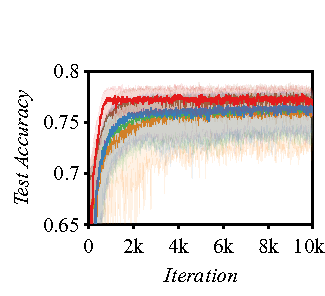
\includegraphics[scale=0.90]{figures/german_02.pdf}
  }  \\
  %% \subfloat[\texttt{heart}]{
  %%   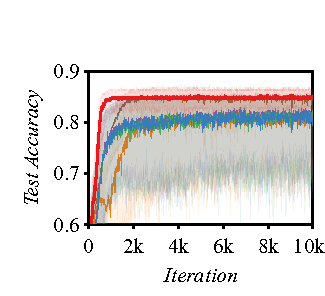
\includegraphics[scale=0.75]{figures/heart_02.pdf}
  %% }
  %% \subfloat[\texttt{german}]{
  %%   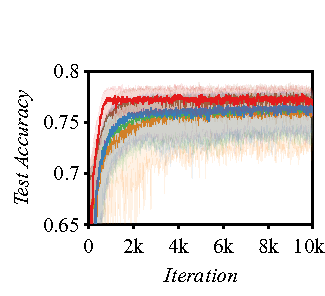
\includegraphics[scale=0.75]{figures/german_02.pdf}
  %% }
  \subfloat[Test Log Predictive Density]{
    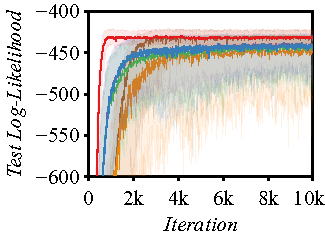
\includegraphics[scale=0.90]{figures/german_03.pdf}
  }
  \caption{Test accuracy and log predictive density on the \texttt{german} dataset.
    The solid lines and colored regions are the mean and 80\% bootstrap confidence interval.
  }\label{fig:logistic}
  \vspace{-0.1in}
\end{figure}
%
\paragraph{Inclusive VI v.s. Exclusive VI}
The results of~\cref{fig:logistic} might be misleading to conclude that inclusive and exclusive VI deliver similar results.
However, in the parameter space, they choose different optimization paths.
This is shown in~\cref{fig:logistic}.
While the test accuracy suggests that ELBO converges around \(t=2000\), in terms of Pareto-\(\widehat{k}\), it takes much longer to converge (about \(t=5000\)).
This shows that, even if their predictive performance is similar, the inclusive VI chooses paths that have better density coverage as expected.

\subsection{Gaussian Process Classification}\label{section:bgp}
%
\begin{figure}[H]
  \centering
  \subfloat[\texttt{sonar}]{
    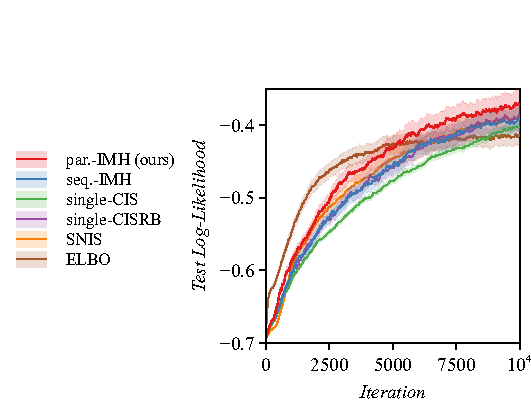
\includegraphics[scale=0.75]{figures/sonar_01.pdf}
  }
  %% \subfloat[\texttt{german}]{
  %%   \includegraphics[scale=0.75]{figures/breast_01.pdf}
  %% } \\
  \caption{Test accuracy and log-likelihood of logistic regression problems.
    The solid lines and colored regions are the medians and 80\% percentiles computed from 100 repetitions.
  }\label{fig:logistic}
\end{figure}
%

\begin{table*}
  \vspace{-0.2in}
  \centering
  \caption{Test Log Predictive Density on Gaussian Process Logistic Classification}\label{table:gp}
  \vspace{-0.05in}
  \setlength{\tabcolsep}{4pt}
  \begin{threeparttable}
  \begin{tabular}{lrrrrrr}
    \toprule
    & \multicolumn{1}{c}{\multirow{2}{*}{ELBO}} & \multicolumn{1}{c}{\multirow{1}{*}{\textbf{pMCSA}}} & \multicolumn{1}{c}{\multirow{2}{*}{JSA}} & \multicolumn{1}{c}{\multirow{2}{*}{CIS}} & \multicolumn{1}{c}{\multirow{2}{*}{CIS-RB}} & \multicolumn{1}{c}{\multirow{2}{*}{SNIS}} \\
    & & \multicolumn{1}{c}{\textbf{(ours)}} & & & & \\
    \midrule
    \textsf{sonar} & {-0.69 {\scriptsize{\(\pm 0.00\)}}} & {\bf-0.68 {\scriptsize{\(\pm 0.00\)}}} & {\bf-0.68 {\scriptsize{\(\pm 0.00\)}}} & {\bf-0.68 {\scriptsize{\(\pm 0.00\)}}} & {\bf-0.68 {\scriptsize{\(\pm 0.00\)}}} & {-0.69 {\scriptsize{\(\pm 0.00\)}}} \\
    \textsf{ionosphere} & {-0.36 {\scriptsize{\(\pm 0.01\)}}} & {\bf-0.35 {\scriptsize{\(\pm 0.01\)}}} & {\bf-0.35 {\scriptsize{\(\pm 0.01\)}}} & {\bf-0.35 {\scriptsize{\(\pm 0.01\)}}} & {\bf-0.35 {\scriptsize{\(\pm 0.01\)}}} & {\bf-0.35 {\scriptsize{\(\pm 0.01\)}}} \\
    \textsf{breast} & {\bf-0.10 {\scriptsize{\(\pm 0.00\)}}} & {-0.11 {\scriptsize{\(\pm 0.01\)}}} & {-0.14 {\scriptsize{\(\pm 0.01\)}}} & {-0.14 {\scriptsize{\(\pm 0.00\)}}} & {-0.14 {\scriptsize{\(\pm 0.01\)}}} & {-0.14 {\scriptsize{\(\pm 0.01\)}}} \\
    \textsf{heart} & {-0.44 {\scriptsize{\(\pm 0.01\)}}} & {\bf-0.43 {\scriptsize{\(\pm 0.01\)}}} & {\bf-0.43 {\scriptsize{\(\pm 0.01\)}}} & {\bf-0.43 {\scriptsize{\(\pm 0.01\)}}} & {\bf-0.43 {\scriptsize{\(\pm 0.01\)}}} & {-0.44 {\scriptsize{\(\pm 0.01\)}}} \\
    \textsf{german} & {\bf-0.48 {\scriptsize{\(\pm 0.01\)}}} & {-0.49 {\scriptsize{\(\pm 0.01\)}}} & {-0.50 {\scriptsize{\(\pm 0.01\)}}} & {-0.50 {\scriptsize{\(\pm 0.01\)}}} & {-0.51 {\scriptsize{\(\pm 0.02\)}}} & {-0.49 {\scriptsize{\(\pm 0.01\)}}} \\
    \textsf{australian} & {\bf-0.21 {\scriptsize{\(\pm 0.01\)}}} & {\bf-0.21 {\scriptsize{\(\pm 0.01\)}}} & {\bf-0.21 {\scriptsize{\(\pm 0.01\)}}} & {\bf-0.21 {\scriptsize{\(\pm 0.01\)}}} & {-0.22 {\scriptsize{\(\pm 0.01\)}}} & {\bf-0.21 {\scriptsize{\(\pm 0.01\)}}} \\\bottomrule
  \end{tabular}
  \begin{tablenotes}
    \item[]{\footnotesize \(\pm\) denotes the 95\% bootstrap confidence intervals obtained from 20 repetitions.}
  \end{tablenotes}
  \end{threeparttable}
  \vspace{-0.15in}
\end{table*}

%%% Local Variables:
%%% TeX-master: "master"
%%% End:

%
\paragraph{Experimental Setup}
Now for a more challenging problem, we perform classification with latent Gaussian processes~\citep{rasmussen_gaussian_2006, NIPS2014_8c6744c9}.
The probabililistic model is given as
\begin{align*}
  \log \vtheta &\sim \mathcal{N}(\mathbf{0}, \mI) \\
   f &\sim \mathcal{GP}\left(\mathbf{0}, \mSigma_{\vtheta}\right) \\
   y_i &\sim \text{Bernoulli-Logit}\left(  f\left( \vx_i \right) \right)
\end{align*}
where we chose a Mat\'ern 5/2 covariance kernel with automatic relevance detection~\citep{neal_bayesian_1996}.
For the datasets, we use the sonar classification (\textbf{\texttt{sonar}}, \(\vz \in \mathbb{R}^{249}\),~\citealt{gorman_analysis_1988}), ionosphere (\textbf{\texttt{ionosphere}}, \(\vz \in \mathbb{R}^{351}\),~\citealt{Sigillito1989ClassificationOR}), and breast cancer (\textbf{\texttt{breast}}, \(\vz \in \mathbb{R}^{523}\),~\citealt{wolberg_multisurface_1990}) datasets.
For \texttt{breast}, we preprocessed the input features with z-standardization.
10\% of the data points were randomly selected in each of the 100 repetitions as test data.
For this experiment, the iteration complexity of ELBO is almost two orders of magnitude larger than all inclusive KL minimization methods.

\paragraph{Result}
The results are shown in~\cref{fig:logistic}.
We can clearly see that among inclusive variational methods, the parallel state estimator (par.-IMH) converges the fastest.
On the other hand, the performance sequential state estimator (seq.-IMH) is very similar to the CIS kernel with Rao-Blackwellization (single-CISRB).
Meanwhile, in terms of held-out predictive probability, exclusive VI (ELBO) converged quickly to a point where the uncertainty is not well calibrated.
All inclusive VI methods were much better calibrated albeit slower to converge.
This matches the 

\subsection{Marginal Likelihood Estimation}\label{section:mll}
%
\begin{figure}[H]
  %\vspace{-0.1in}
  \centering
  \begin{minipage}[b]{0.3\linewidth}
    \centering
    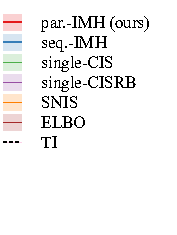
\includegraphics[scale=0.8]{figures/radon_03.pdf}
  \end{minipage}
  \begin{minipage}[b]{0.6\linewidth}
    \centering
    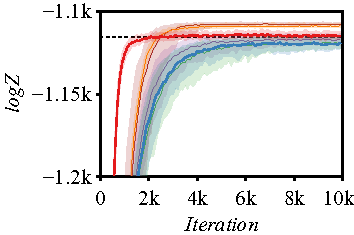
\includegraphics[scale=0.8]{figures/radon_02.pdf}
    \subcaption{\texttt{radon}}
  \end{minipage}
  %% \begin{minipage}[b]{0.35\linewidth}
  %%   \centering
  %%   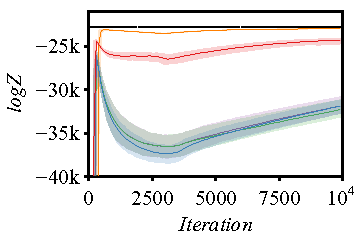
\includegraphics[scale=0.7]{figures/sv_02.pdf}
  %%   \subcaption{\texttt{stock}}\label{fig:sv}
  %% \end{minipage}
  \caption{Marginal log-likelihood (\(\log Z\)) estimates of considered methods.
    The solid lines and colored regions are the medians and 80\% percentiles computed from 100 repetitions.
  }\label{fig:marginal_likelihood}
  %\vspace{-0.15in}
\end{figure}
%
\paragraph{Experimental Setup}
We now estimate the marginal log-likelihood of a hierarchical regression model with partial pooling (\texttt{radon}, \(\vz \in \mathbb{R}^{175}\),~\citealt{gelman_data_2007}) for modeling radon levels in U.S homes.
\texttt{radon} contains multiple posterior degeneracies from the hierarchy.
We estimated the reference marginal likelihood using \textit{thermodynamic integration} (TI,~\citealt{gelman_simulating_1998, neal_annealed_2001, lartillot_computing_2006}) with HMC implemented by Stan~\citep{carpenter_stan_2017, betancourt_conceptual_2017}.

\paragraph{Results}
The results are shown in~\cref{fig:marginal_likelihood}.
On \texttt{radon}, MSC-PIMH converges quickly and provides the most accurate estimate.
By contrast, MSC-CIS and MSC-CISRB converge much slowly.
SNIS and ELBO, on the other hand, overestimate \(\log Z\), which can be attributed to the mode-seeking behavior of ELBO and the small sample bias of SNIS.


%%% Local Variables:
%%% TeX-master: "master"
%%% End:
